\documentclass[../thesis]{subfiles}

\begin{document}

\chapter{Implementation}


The complete eGor system is a distributed application consisting of
numerous software components running on several different
computers. To manage this complexity, the developers have attempted to
make disciplined use of best practices for web programming and to make
judicious use of a range of cutting-edge third party libraries, only
accepting those which have a record of stability and continued
maintenance.

Our complete system draws on a wide range of technologies from every
level of the software stack. This chapter provides a description of
what new components were implemented by the project's development
team, which external tools and libraries were used, and what
architectural and practical concerns factored into the selection of
these methods. This is intended to provide an overall understanding of
how the application is structured rather than detailed developer
documentation, which can be found at
\url{https://github.com/egor-elab/doc}.



\section{Overview}

Figure \ref{fig:ImplOverview} shows a high-level schematic of the
current structure of the eGor platform. The components depicted are
divided across three different machines in the simplest scenario,
although more complex configurations are possible since all services
interact over network-ready protocols such as HTTP. These machines
are, from top to bottom
\begin{enumerate*}[label=(\roman*)]
  \item{
      the end-user's PC, where an interactive single-page browser
      application is used to interact with various eGor services
      graphically,
  }
  \item{
      a server running microservices for functions such as
      authentication, remotely accessible persistent data storage, and
      routing requests to other services and digital resources, and
  }
  \item{
      one or more machines physically connected to scientific
      equipment of interest, responsible for managing and issuing
      commands to appropriate device drivers.
  }
\end{enumerate*}

\begin{figure}
  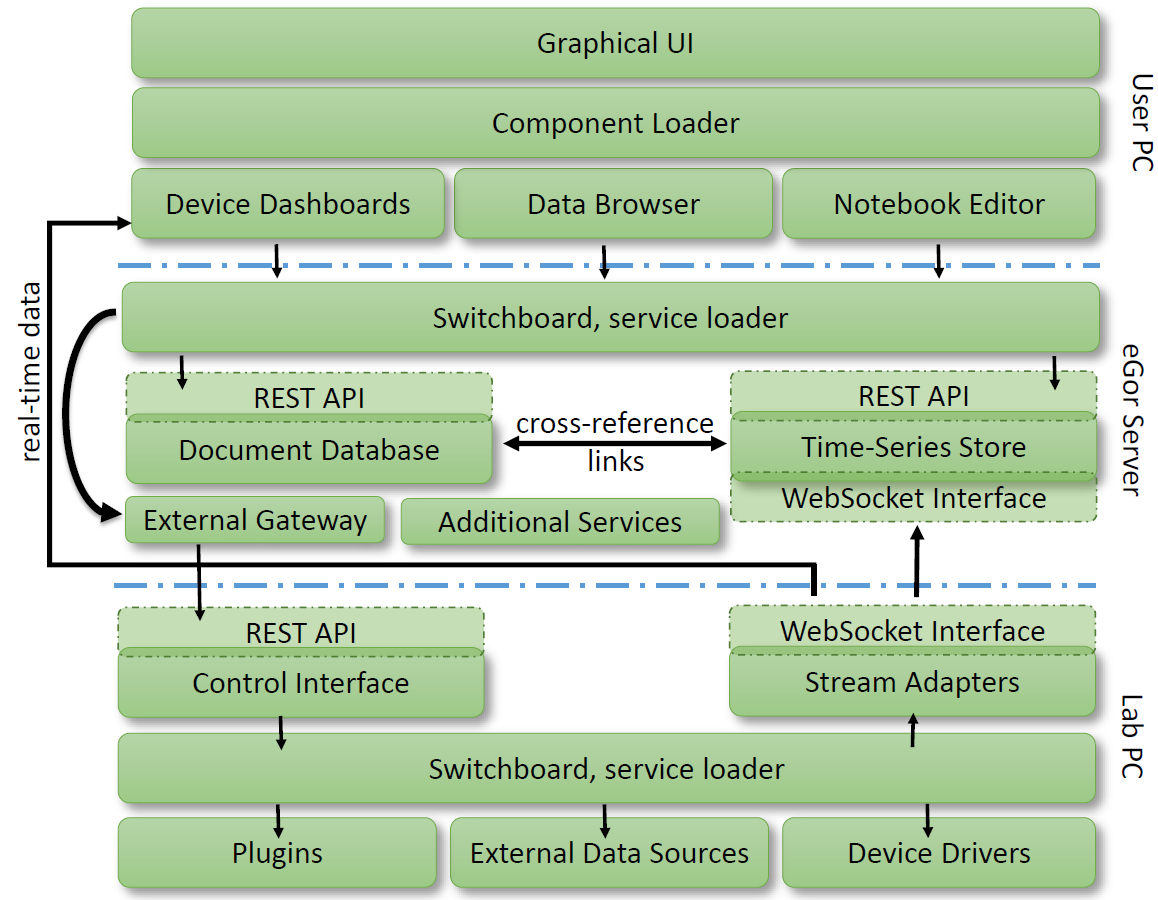
\includegraphics[width=\textwidth]{impl-overview}
  \caption{
    A high-level architectural view of the implemented eGor system,
    divided across three different machines where primary activity
    takes place: a user's machine, connected to an eGor server via a
    web browser, which issues commands to a lab PC running device
    management services to connect with lab equipment.
    \label{fig:ImplOverview}
  }
\end{figure}

This chapter will elaborate the organization and communication
strategies used to implement this framework in software, followed by a
technical discussion of each component's internals.  Other than the
in-browser graphical interface, which is written as a single-page
application in HTML5 and JavaScript using the Angular framework
\cite{Angular}, the majority of the eGor web application is written in
Python \cite{Python}, making use of the mature and modern palette of
networking and communications libraries available in the language. An
important exception is found in some portions of the database access
layer, which use NodeJS \cite{NodeJS} libraries to present a simple
and effective API. The user-facing web application structure uses all
the major third party components of the popular MEAN stack \cite{MEAN}
(MongoDB, ExpressJS, AngularJS, and NodeJS), but interacts with
several Python microservices to add hardware
connectivity.

Additionally, the eGor team has developed a model
embedded device to help demonstrate how physical actuators and data
acquisition modules might interact with the system -- the software for
this target is written in C++. This device, known as aMEASURE I, is intended to
act as a flexible instrument for performing electrochemical
experiments and recordings and lies outside the scope of the eGor project
proper, but throughout this chapter we use it as a concrete example of
the kind of device the framework supports. aMEASURE I can store and
produce arbitrary waveforms by a number of methods, record
digitally-converted analog measurements and stream them over a serial
interface in real-time, and interact with external circuits via banks
of I/O pins.

The software for all these core
components is open-source and available in several Git repositories
hosted at \url{https://github.com/egor-elab}. The diverse set of
languages used helps to demonstrate a chief strength of eGor's
microservice architecture: components are sufficiently decoupled that
they can individually be implemented in a language and style
well-suited to their unique challenges.

\subsection{Design principles}
Over the course of developing and refining the eGor toolchain, several
recurring patterns have emerged which seem natural fits for addressing
the application's goals and have informed subsequent iterations of the
design. This section discusses several key \glspl{designPattern} which have
been observed and employed throughout the code base, providing a feel
for the philosophy of the complete system before delving into
implementation details.

\subsubsection{Request/Response vs. Publish/Subscribe}
The most common form of high-level network traffic on the web is HTTP,
which uses request/response exchanges to pass data between hosts. For
instance, a client such as a web browser might issue an HTTP request
to a server with the contents \texttt{GET /users}, causing the server
to respond with a text payload encoding a resource named
``\texttt{users}''. The client submits user input such as form data in
a similar way (typically via an HTTP \texttt{POST} action), resulting
in an acknowledgment message from the server. This approach is
sufficiently flexible to allow for much of the broad range of content
found on the modern web, especially since servers often deliver
JavaScript source code for clients to execute locally in addition to
static text documents such as HTML. Issuing commands to lab equipment
can often be modeled in a similar way: a controlling computer submits
a configuration message and the device responds with a (possibly
empty) acknowledgment that the command was received and executed.  In
many ways these operations are also analogous to the ubiquitous
programming construct of calling a subroutine, and some authors place
transactions such as HTTP actions under the umbrella of \glspl{RPC}
\cite{DBLP:journals/corr/abs-0911-4395}.

Request-and-response communication is, however, a poor fit for systems
where communications must be initiated bidirectionally, with
event-driven applications providing a key example. A typical
data-collecting lab instrument or digital microsystem produces values
in real time which must be transmitted to destinations such as
databases and display monitors at roughly the same rate as they are
captured. Implementations can still accommodate this dataflow into a
request/response framework by periodically requesting buffers from the
data source, but this approach is fraught with difficulties and is
typically complicated to use when many data sources need to be managed
simultaneously.

A more elegant \gls{designPattern} for systems with soft real-time
requirements is given by the publish/subscribe approach, also
sometimes called the Observer pattern \cite{GangOfFour}. In this
scheme, a ``topic'' or ``observable'' object maintains a list of
``subscribers'', and notifies each of them when a variable of interest
changes or an event is ``published'' to the event stream. The
publish/subscribe technique has been adopted to solve software
problems like real-time data acquisition as well as for building
``reactive'' applications such as user interfaces and games, where
graphical interfaces are expected to react seamlessly to event streams
such as user input and network communications. eGor adopts this
pattern for both these use cases, treating data collection devices as
publishers of streams of data fragments which may be subscribed to by
other services or graphical interfaces throughout the system.

\subsubsection{Dynamic loading}
One of the chief observations underpinning eGor's design is that
researchers' needs are too diverse and rapidly changing to be
satisfactorily addressed by a single rigidly constructed
application. The implementation effort has therefore focused on
constructing a core infrastructure which allows future developers to
easily integrate new functionality without disturbing the system's
overall operation. Each major component of eGor allows its users to
load new extensions at runtime. The core subsystems each specify an
interface for how a module should allow itself to be installed and
expose its functionality to the network, and otherwise
community-contributed extensions are not required to depend on eGor
APIs or even to be written in the same programming language as the
rest of the framework.

In addition to being an essential part of the daily workflow for
eGor's developers, a distributed version control system (namely Git
\cite{Git}) provides a runtime mechanism for achieving this dynamic
loading functionality. Git was designed to allow many programmers to
collaborate on a software project, share contributions remotely, and
review and revert changes. Importantly, Git is distributed in the
sense that each user may maintain an independent timeline of the
history of the code base on a private computer, with or without
network connectivity, sharing or publishing changes in a peer-to-peer
fashion if and when they choose.

An example of the dynamic loading process is illustrated in figure
\ref{fig:DynamicLoading}. The following sequence of steps describes
how, for instance, the device management system might \glspl{lazyLoad} a
device driver, waiting to download and install the appropriate code
until the device has been physically connected to a given host machine
for the first time. Here the phases are listed with the same numbering
as in figure \ref{fig:DynamicLoading}.

\begin{enumerate}
  \item{
      A client service attempts to access functionality on another
      service which is not presently running, or explicitly requests for
      a new service to be loaded. In this case, the client is a service
      responsible for enumerating the serial ports available on the
      system and attempting to retrieve identifying information from
      connected devices, and its request for a device driver includes
      identifying information but may not name the driver explicitly.
  }
  \item{
      The ``service-hosting service'', responsible for managing
      dynamically loaded programs, queries a database of service
      information to determine where it can download the requested
      code. The database responds with a \gls{URI} specifying either a
      direct link to the necessary files or a Git repository.
  }
  \item{
      The service-hoster downloads the module, possibly from an
      internal server or from a publicly hosted location such as
      Github \cite{Github}, and executes necessary startup
      routines. If the service-hoster determines that the service is
      already loaded, it instead checks if an updated version exists
      and provides the client with the option to download and use the
      new version. eGor services are expected to implement a common
      interface of setup, start, stop, and cleanup scripts so that the
      service-hoster can install and run them automatically. The
      service-hoster also indicates to the new service instance how it
      can communicate with the system switchboard responsible for
      triggering the download.
  }
  \item{
      Once the dynamically loaded device driver is live, it registers its
      public \gls{API} with the switchboard, at which point the
      driver's functionality is available for other services to use.
  }
  \item{
      The switchboard completes any pending procedure calls requested
      by the client service, and routes subsequent requests to the
      appropriate service.
  }
\end{enumerate}

A similar procedure is employed for several other
subsystems, such as loading new user interface components or adding
new waveform generation routines to our real-time electrochemical
interrogation platform.

\begin{figure}
  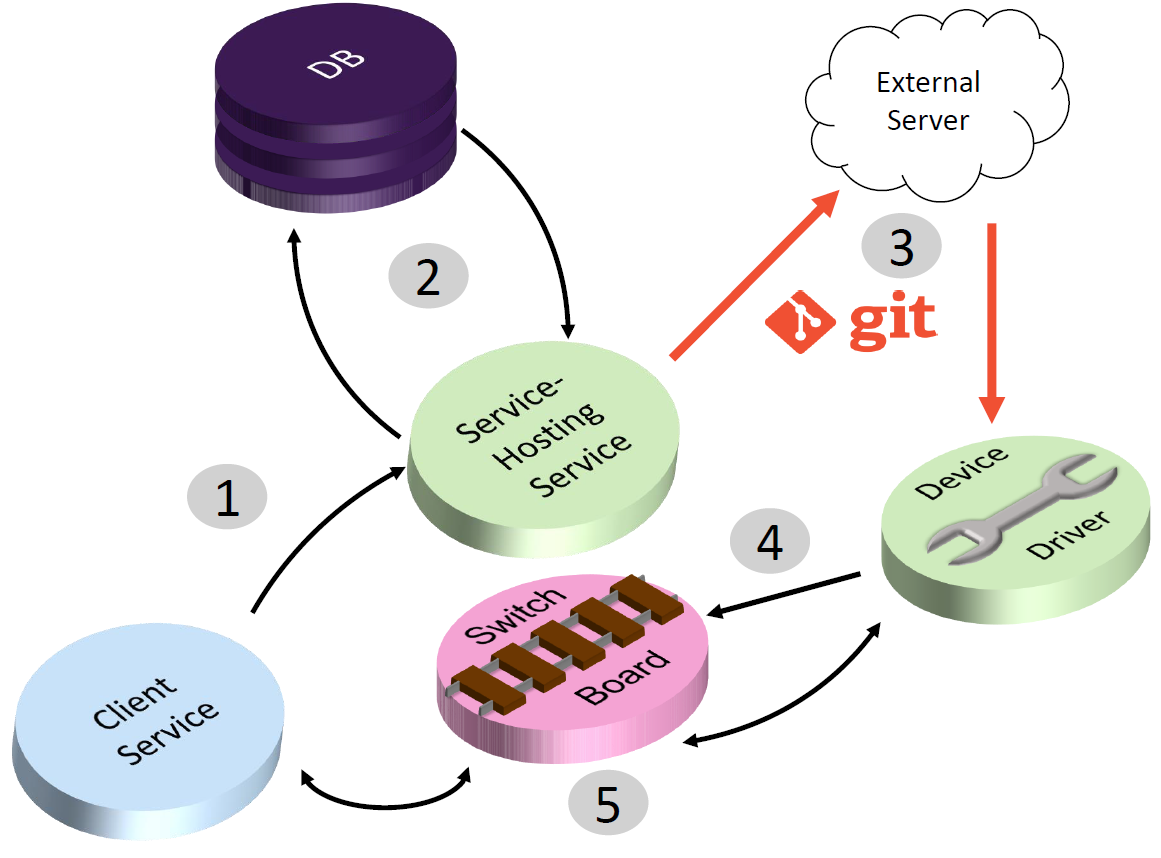
\includegraphics[width=\textwidth]{dynamic-loading}
  \caption{
    Phases of the dynamic loading process for downloading and
    installing a user-defined device driver at runtime. The
    service-hosting service and the services it hosts (green)
    run on the same physical hardware, whereas each other service may
    be on a different device connected via the Internet.
    \label{fig:DynamicLoading}
  }
\end{figure}

\subsection{Implementation status}



\section{Service interconnect}
As described in Chapter 3, the microservice architectural pattern
provides a strategy for compartmentalizing the development effort,
promoting modularity of design, allowing for future customization and
extension, and building a system that employs many different software
technologies and physical machines. However, communication between
microservices involves some challenges compared to traditional
architectures and relies on several recently emerged web technologies
to allow services to locate and use one another. Nonetheless,
the microservice approach pairs well with eGor's high-level goals and
has enabled us to build a flexible and sophisticated system.

\subsection{REST APIs}
One of the elements of the web's modern infrastructure that has made
networked microservice-oriented applications a practical possibility
is the widespread adoption by businesses and open-source software
providers of relatively uniform, publicly available \glspl{API} over
HTTP. Most commonly, companies expose reusable public components of
their web servers as HTTP interfaces which aspire to \gls{REST}
principles, i.e., they model the evolution of an application's state
as a sequence of transitions between states which are modeled by
\glspl{URI}. These conventions have allowed for unprecedented
interoperability between applications written at different companies
for very different purposes. As a prominent example, Google's Maps
\gls{API} provides a mechanism for other applications to retrieve
geographical information over an Internet connection rather than
maintaining independent location databases. Given that many consumers
of these APIs are web browser applications which use JavaScript to
issue background HTTP requests, \gls{JSON} is a popular serialization
format for passing data payloads to and from API endpoints. This
structure, where a website provides an indexable collection of
\gls{JSON}-encoded resources which can be retrieved and manipulated
via HTTP verbs, is often what is meant by a \gls{RESTAPI} in today's
software jargon.

\glspl{RESTAPI} are useful interfaces for making application state and
data externally accessible, but are also a viable option for
structuring networked communication between different parts of the
same app. Most commonly, a \gls{RESTAPI} is used to provide structured
database access to client code running in a browser app. For example,
a news website might allow clients to retrieve a list of articles (in
\gls{JSON} format) by making a \texttt{GET /articles} HTTP request,
then retrieve the user's selected document by querying \texttt{GET
  /articles/2}, then commit a submitted comment to the database with
\texttt{POST /articles/2/comments}. Many of the existing tools for
constructing \glspl{RESTAPI} with web programming frameworks such as
Python's Flask \cite{Flask} or Express in NodeJS \cite{Express}
provide for this use case.

In eGor we assign URIs in a similar hierarchical fashion, but the
total application consists of a number of groups of microservices,
each potentially possessing a \gls{RESTAPI}. As new services are
loaded by a particular switchboard, their \glspl{API} are attached to
the tree of existing \glspl{URI}, much as a filesystem on a new hard
drive might be mounted at a particular path on a UNIX filesystem.  An
eGor switchboard achieves this by serving a proxy at a \gls{URI}
corresponding to a known lab machine, such as \texttt{/machines/0},
relaying traffic to and from that machine which in turn provides
access to connected devices as \glspl{RESTAPI} at appropriate
\glspl{URI}. Information about the waveform types that a device called
``aMEASURE I'' is capable of producing would then be available by
accessing \texttt{GET /machines/0/devices/aMEASURE\_I/wave/info},
assuming that the \gls{RESTAPI} for \texttt{aMEASURE\_I} understands
how to interpret the path \texttt{/wave/info}. Specifying a
\gls{RESTAPI} is part of a user's responsibility when defining a
driver for a new device, as explained further in section
\ref{sec:DevDrivers}.

\subsection{WAMP routing}
\gls{WAMP} is an open protocol and software stack definition created
by Tavendo, who provide reference implementations in several languages
in the form of the Autobahn protocol libraries and a request router
called crossbar.io \cite{CrossbarIO}. The authors of these tools claim
that their protocol simultaneously addresses many of the use cases of
existing protocols for machine-to-machine communication such as
\gls{AMQP} and socket.io \cite{socket.io}. The protocol is built on
top of WebSockets, which uses a TCP connection to achieve reliable
full-duplex streaming and is now supported by all major web browsers
and a number of web frameworks in several programming languages. One
advantage provided by this protocol design approach is that machines
for hosting microservices or acting as clients for \gls{WAMP} networks
can require less special software than is required for using some
message queuing infrastructures such as \gls{AMQP}, simplifying the
installation process for end users.

\gls{WAMP} provides a set of capabilities which are a good match for
our application, including built-in support for routing remote
procedure calls between any two connected services and bidirectional
publish/subscribe-style message passing \cite{WAMP}. The protocol was
explicitly designed to simplify the implementation of \gls{IoT}
applications, especially those with service-oriented architectures
that span multiple devices of different types. Furthermore, \gls{WAMP} is
designed to target many different languages and target devices,
providing a common network interface between server-side code,
browsers, and mobile apps, and the abstraction and separation of
concerns provided by such a framework is well-matched to heterogeneous
service-oriented architectures such as eGor's. This provides an
attractive solution for addressing many of the problems faced when
developing our system, especially given that it allows for dynamic
registration and removal of remotely-callable methods, flexible
routing of data sources through different machines and endpoints, and
is inherently bidirectional in the sense that any service can initiate
communication with any other so long as it has sufficient security
privileges. In the existing implementation, \gls{WAMP}'s capabilities
have primarily been used for service-to-service communication and to
organize streaming data transactions from data sources to sinks such
as real-time plots and array storage services. A more elegant and
truly service-oriented design could be achieved by adopting \gls{WAMP}
for issuing user commands and making database accesses as well, but at
the time of this writing \gls{WAMP} has poorer tooling and
documentation than some of its more established counterparts.



\section{User interface}
Providing a useful and manageable interface for scientific users who
are not computer experts is one of eGor's most important design
constraints. The development effort has leveraged several powerful
libraries for developing web applications and providing desired user
interface features to allow researchers to immediately take advantage
of eGor's capabilities.

\subsection{Thin client design}
All graphical interface components of eGor are implemented as
interactive web pages and require only a modern web browser and an
Internet connection to use. In this way the user interface acts as a
\gls{thinClient} portal connecting users to an eGor server. This
approach has the advantage of requiring no installation on the user's
part other than registering an account, as well as making software
updates transparent to users, since the latest version is
automatically retrieved from the server each time a user
connects. Furthermore, our approach implements the user interface as a
single-page application, meaning that a user's entire session takes
place without retrieving more than one page from the server or
refreshing, instead using asynchronous HTTP requests in the background
and bidirectional WebSocket communication to synchronize application
state with the server. Structuring client-server interactions in this
way helps to decouple the browser from the back-end, allowing these
components to be developed independently. By leveraging abstractions
provided by \gls{WAMP}'s application framework, it is possible for
user interface components such as plots and control panels to act as
peers with other microservices, simplifying the structure of the
program.

\subsection{Angular 2}
The JavaScript framework underpinning eGor's browser app \gls{UI} is
Angular 2, a complete rewrite of the popular and sophisticated
AngularJS framework for building single-page applications
\cite{Angular}. Angular gives programmers a toolkit for defining
custom HTML5 tags with dynamic behavior and for ``two-way data
binding'' between elements of a web page and JavaScript objects. This
means that display elements are automatically updated when specified
JavaScript variables change, and similarly user inputs such as changes
to form elements are automatically reflected in bound JavaScript data
structures. This synchronization between elements of a page's
\gls{DOM} and corresponding variables in the JavaScript program allows
for a \gls{declarative} programming style to be used to describe how
an app is displayed while writing the control logic with sequential,
imperative JavaScript.

Advantages of Angular 2 over its predecessor and other client-side
programming frameworks include a structured, object-oriented style, a
focus on reactive programming using the Observer pattern, and improved
support for asynchronous functionality such as \gls{lazyLoad}ing
components and application structure. In particular, the
\glspl{designPattern} embraced by Angular allow eGor's developers to
carry a modular, service-oriented philosophy through to the user
interface, compartmentalizing functionality into a connected group of
independent, dynamically loaded services.

\subsection{UI components on demand}
Although Angular is built for creating single-page browser
applications, their associated JavaScript code often makes many
behind-the-scenes network requests to retrieve requested or up-to-date
information. A map application provides a familiar example: rather
than loading geographical information about the entire globe when the
page is first loaded, new connections to \glspl{RESTAPI} are made
asynchronously in the background to retrieve more data as the user
pans and zooms the map to view different locations. In addition to
providing full-featured abstractions for retrieving and managing
remote data sources of this kind, Angular 2 has capabilities for
dynamically loading application code as well. A typical use-case for
this feature is to \gls{lazyLoad} components that do not need to be
present in the page initially, reducing startup time by waiting to
download some JavaScript modules or HTML templates until the user
navigates to a state which requires them.

eGor's design makes use of this dynamic loading functionality to allow
for arbitrary extensions to the \gls{UI}. Each document stored
in eGor's artifact database may be associated with one or more
\gls{UI} components, self-contained Angular modules which provide
special-purpose functionality associated to a user, device, or
experiment. For instance, the aMEASURE I electrochemical measurement
device provides a real-time data monitor and several control panels
corresponding to the different waveform generation mechanisms it
supports. The database record storing information about this
device contains an entry for each of these \gls{UI} widgets including
links to JavaScript code defining an Angular component and its
business logic, HTML and CSS files declaring how they should be
displayed, and links to additional asset files such as images and PDF
operator's manuals.

As with other elements of the eGor framework that employ dynamic
loading, this design allows the core software to remain small,
efficient, and single-purpose while allowing future developers and
users to create and customize components to meet their needs.  By
choosing \gls{WAMP} as the network interconnect between services, we
have also made it possible for JavaScript components in the browser to
interact with back-end services over the same communication interface
as the microservices use with each other, promoting scalability and
modular design. This component-based approach to building the browser
app could be supplemented by a graphical tool allowing users to
drag-and-drop interface components to build their ideal control panel
in a similar way that users of LabVIEW are accustomed to constructing
control panels for their virtual instruments \cite{LabVIEW}. This
approach also aligns with our microservice architecture, where
functionality is contained in independent interacting components which
may have very different internal behaviors. The decoupled design also
allows the system to embed third-party web components and even
entirely different browser apps into the front-end, enabling eGor to
integrate existing open-source software packages such as electronic lab
notebooks with our design.

\subsection{Jupyter}
The Jupyter project (formerly IPython) is an open-source software tool
providing a flexible architecture for creating electronic lab
notebooks for scientific computing. Jupyter now supports many of the
most popular programming languages for science and engineering
applications and has several extension packages providing additional
functionality, most notably JupyterHub. JupyterHub provides a web
server which allows teams to share and collaboratively edit notebooks
in the browser, embedding plots, equations, code and more inside a
document that doubles as an executable analysis program. This tool is
well-supported and has addressed many of the important challenges
associated with building a collaborative documentation tool for
computational science.

eGor experiment artifact model includes a \gls{UI} component called
``Notebook'' which embeds a Jupyter Python notebook inside the eGor
browser app. This allows researchers to attach analysis and
observations to an experiment in a flexible format using a
full-featured language and toolkit for scientific computing. Since
many eGor components were developed with Python, this also provides a
mechanism for users to interact directly with other system components
at many levels of abstraction, potentially interleaving instrument
control commands and signal processing in a single notebook. Python
libraries such as Numpy \cite{Numpy} or Pandas \cite{Pandas} also
provide powerful high-level APIs for interacting with data sets, and
eGor provides access to an experiment's raw data files from within the
associated Jupyter notebook. This approach uses a mature program to supplement
eGor with much-needed \gls{ELN} functionality and demonstrates
how the modular design allows for embedding useful third-party tools
into the browser app.



\section{Database management}
A careful choice and implementation of the system's data model is
important for performance, flexibility, and determining the
organization of the app. eGor employs multiple server-side data stores
for persisting datasets, images and documents, information about
experiments, devices, and users, and records describing eGor
components such as code for dynamically loaded modules.

\subsection{NoSQL and schemaless databases}
For many years web applications primarily used relational databases
for persistent data storage, querying and assembling them using
\gls{SQL}. These databases are based on well-understood theoretical
foundations and have a number of advantages for applications such as
business operations management and traditional web architectures, but
have performance difficulties when dealing with complex data
structures that are not naturally suited to a table format
\cite{Mohan:2013:HRI:2452376.2452378}. Relational databases are often
also rigidly tied to a \gls{databaseSchema}, making them ill-suited
for records with many small variations in structure or with structures
that change over time.

In response to the difficulties posed by this technology, considerable
investment has been made in recent years in developing alternative
database styles which offer more flexibility and parallel
scalability. The primary information of interest to eGor is complexly
structured and chiefly concerned with relationships between
publications, experiments, data sets, and devices, and we sought to
adopt a database technology capable of naturally modeling these
artifacts and their connections. For this reason we initially examined
graph databases and relational database representations of semantic
web content, but ultimately chose the document database MongoDB to
reflect the nested, inheritance-focused structure of our data
model. MongoDB's internal structures also map directly to the
\gls{JSON} object structure used for communication and state
representation throughout the eGor system. The popularity of document
databases in the NodeJS ecosystem has created a thriving space of
open-source tools for working with systems like MongoDB and connecting
them to other important application components

Constructing an \gls{API} layer to expose \gls{REST}ful access to a
database involves a substantial amount of boilerplate and can become
quite error-prone and difficult to manage as system and data model
complexity increases. StrongLoop LoopBack \cite{LoopBack} is an
open-source framework which generates \gls{API} endpoints and
documentation for one or more server-side data stores.
LoopBack is built on top of the NodeJS web application framework
ExpressJS, allowing it to be used in conjunction with the wide array of
community plugins and middlewares available for Express. In eGor,
LoopBack is used to produce object models for artifacts such as
instruments, virtual workbenches, experimental runs, result sets, and
eGor software plugins. LoopBack generates hand-customizable
\glspl{RESTAPI} for declaratively defined data models, automatically
handles accesses to several different database backends,
and includes application logic for important fundamental tasks such as
access controls, account creation, and file uploads.

\subsection{HDF5}
Although NoSQL databases such as MongoDB provide a flexible solution
for persistent storage of complex document-like data, they are
ill-suited for efficiently querying large array-like scientific data
sets. HDF5 is a technology for manipulating multidimensional
time-indexed formats that has seen strong adoption in the finance, machine
learning, and data science fields in recent years \cite{HDF5}. The
open source working group responsible for developing the HDF5
specification has also provided a Python web server for storing
datasets and presenting them as network resources, which includes a
reference implementation of a REST API for remotely manipulating
and extracting subsets of datasets.


\section{Device management}
eGor's core framework includes a microservice which runs on an
instrument-connected lab PC and is responsible for detecting which
instruments are connected, loading appropriate device drivers and
protocol-translating software modules, and presenting a uniform
network interface for handling device controls and data in the form
of \gls{REST} and \gls{WAMP} \glspl{API}. This section discusses the
design of the instrument management service (written in Python) and
explains how some of the challenges in its implementation were
addressed.

\subsection{Enumeration}
One complication that arises when attempting to communicate with many
different lab devices is that it is difficult for a PC to determine
exactly which devices are connected to it. Many scientific instruments
use legacy protocols and hardware such as serial or parallel ports
which provide no built-in mechanism for identifying a device or its
capabilities to a host machine. To address this problem, the
measurement equipment industry standardized the \gls{VISA} \gls{API},
which is implemented by instruments from a number of different
manufacturers \cite{VISA}. To determine what device is connected and
load an appropriate device driver, the host must send a message to the
instrument asking for identifying information.

Typically serial instruments are connected to modern PCs using
USB-to-serial adapters. Further complicating the enumeration process,
information provided to user-space applications about USB connected
devices and USB connection events varies by operating system and does
not necessarily contain information about whether a given USB device
is a serial port. The eGor microservice responsible for tracking
connected devices therefore uses the following algorithm to keep an
up-to-date record of which equipment is connected.

\begin{enumerate}
  \item{
      When a USB event occurs signaling connection or disconnection of
      a device, the instrument manager triggers a re-scan of all
      serial ports.
  }
  \item{
      To scan a given port, the instrument manager transmits the
      \gls{VISA} identification command ``\texttt{*IDN?}'' and waits
      for a response. Since the communication rate of the target
      device is unknown, this step must sequence through a list of
      commonly used baudrates, pausing after each transmission to see
      if a response is received. Since some devices of interest to not
      conform to the \gls{VISA} specification, different
      identification messages are transmitted to probe for some
      other known devices.
  }
  \item{
      Once a response is received to an identification request, the
      database is queried with the instrument's response string and
      the baudrate that was used to retrieve it. The database is
      searched for a known device driver matching this profile.
  }
  \item{
      If an appropriate device profile is found, the service-hosting service
      on the lab PC is asked to download and install the microservice
      used to manage interaction with the target device.
  }
  \item{
      The device driver microservice is brought up, issues startup
      commands to the device, and registers its high-level \gls{API}
      with the eGor switchboard.
  }
\end{enumerate}

\subsection{Protocol stacks}
One of the most important capabilities of the eGor system is its
ability to connect to computer-controlled lab equipment. Scientific
processes often involve a wide range of legacy instruments which use
different communication protocols and data formats. Rather than
attempting to provide individual drivers and protocol translators for
the many devices that our future users may need, we have constructed a
Python library of simple protocol building blocks which can be
connected into more elaborate protocol stacks.

We abstractly define a protocol layer as a composable software unit
for transforming units of data from one format to another. A protocol
layer consists of a codec, a transport, and a controller. One or more
of these subcomponents may inherit the default implementation from the
``layer'' base class, which simply passes data through
unaltered. These layers


\subsection{Writing drivers} \label{sec:DeviceDrivers}

\section{Summary}





\end{document}
